\section{Summary of findings}
\label{sec:summary-findings}

This section discusses the security problems identified for this scenario and our proposed mitigations.

\subsection{Architectural changes}

Figure \ref{fig:updated-network} shows our proposal in updating the network architecture in order to better suit modern standards and also to increase resiliency to attacks. These measures are the first and foremost that should be undertaken, and must go hand in hand with the countermeasures proposed in our qualitative and quantitative analysis in the next sections.

\begin{figure}[!h]
	\centering
	%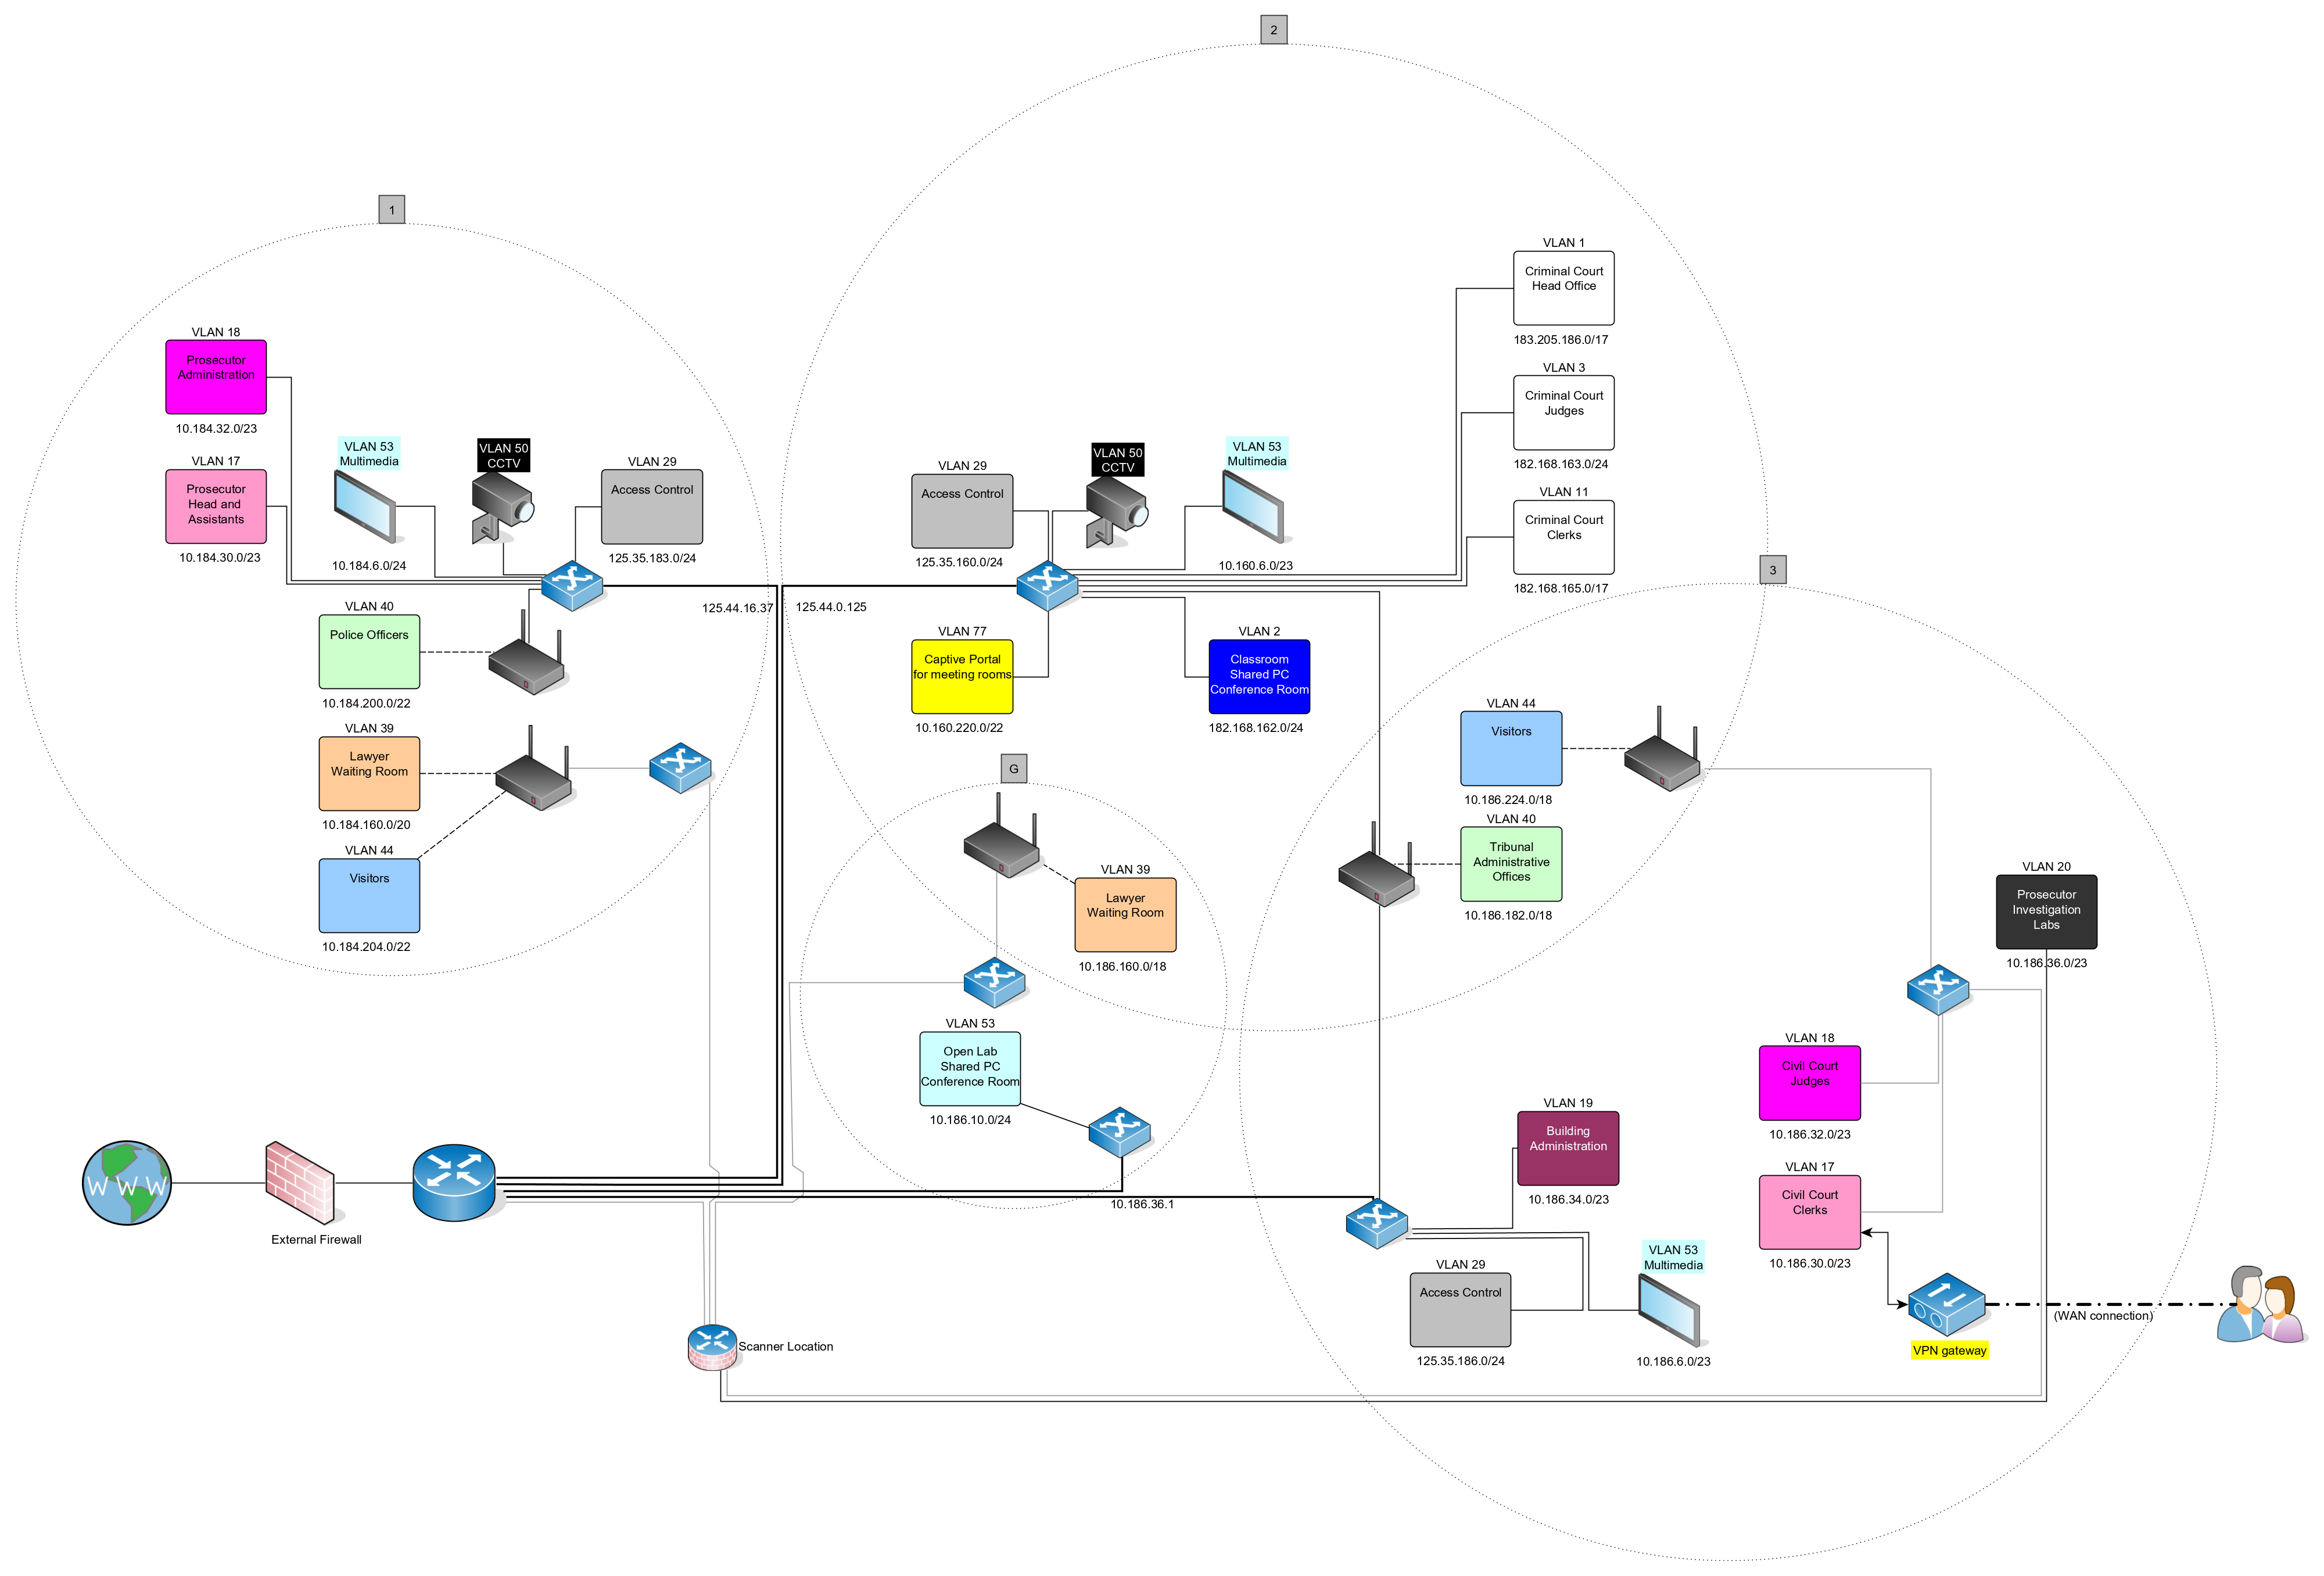
\includegraphics[width=1.4\textwidth]{drawable/rete.png}
	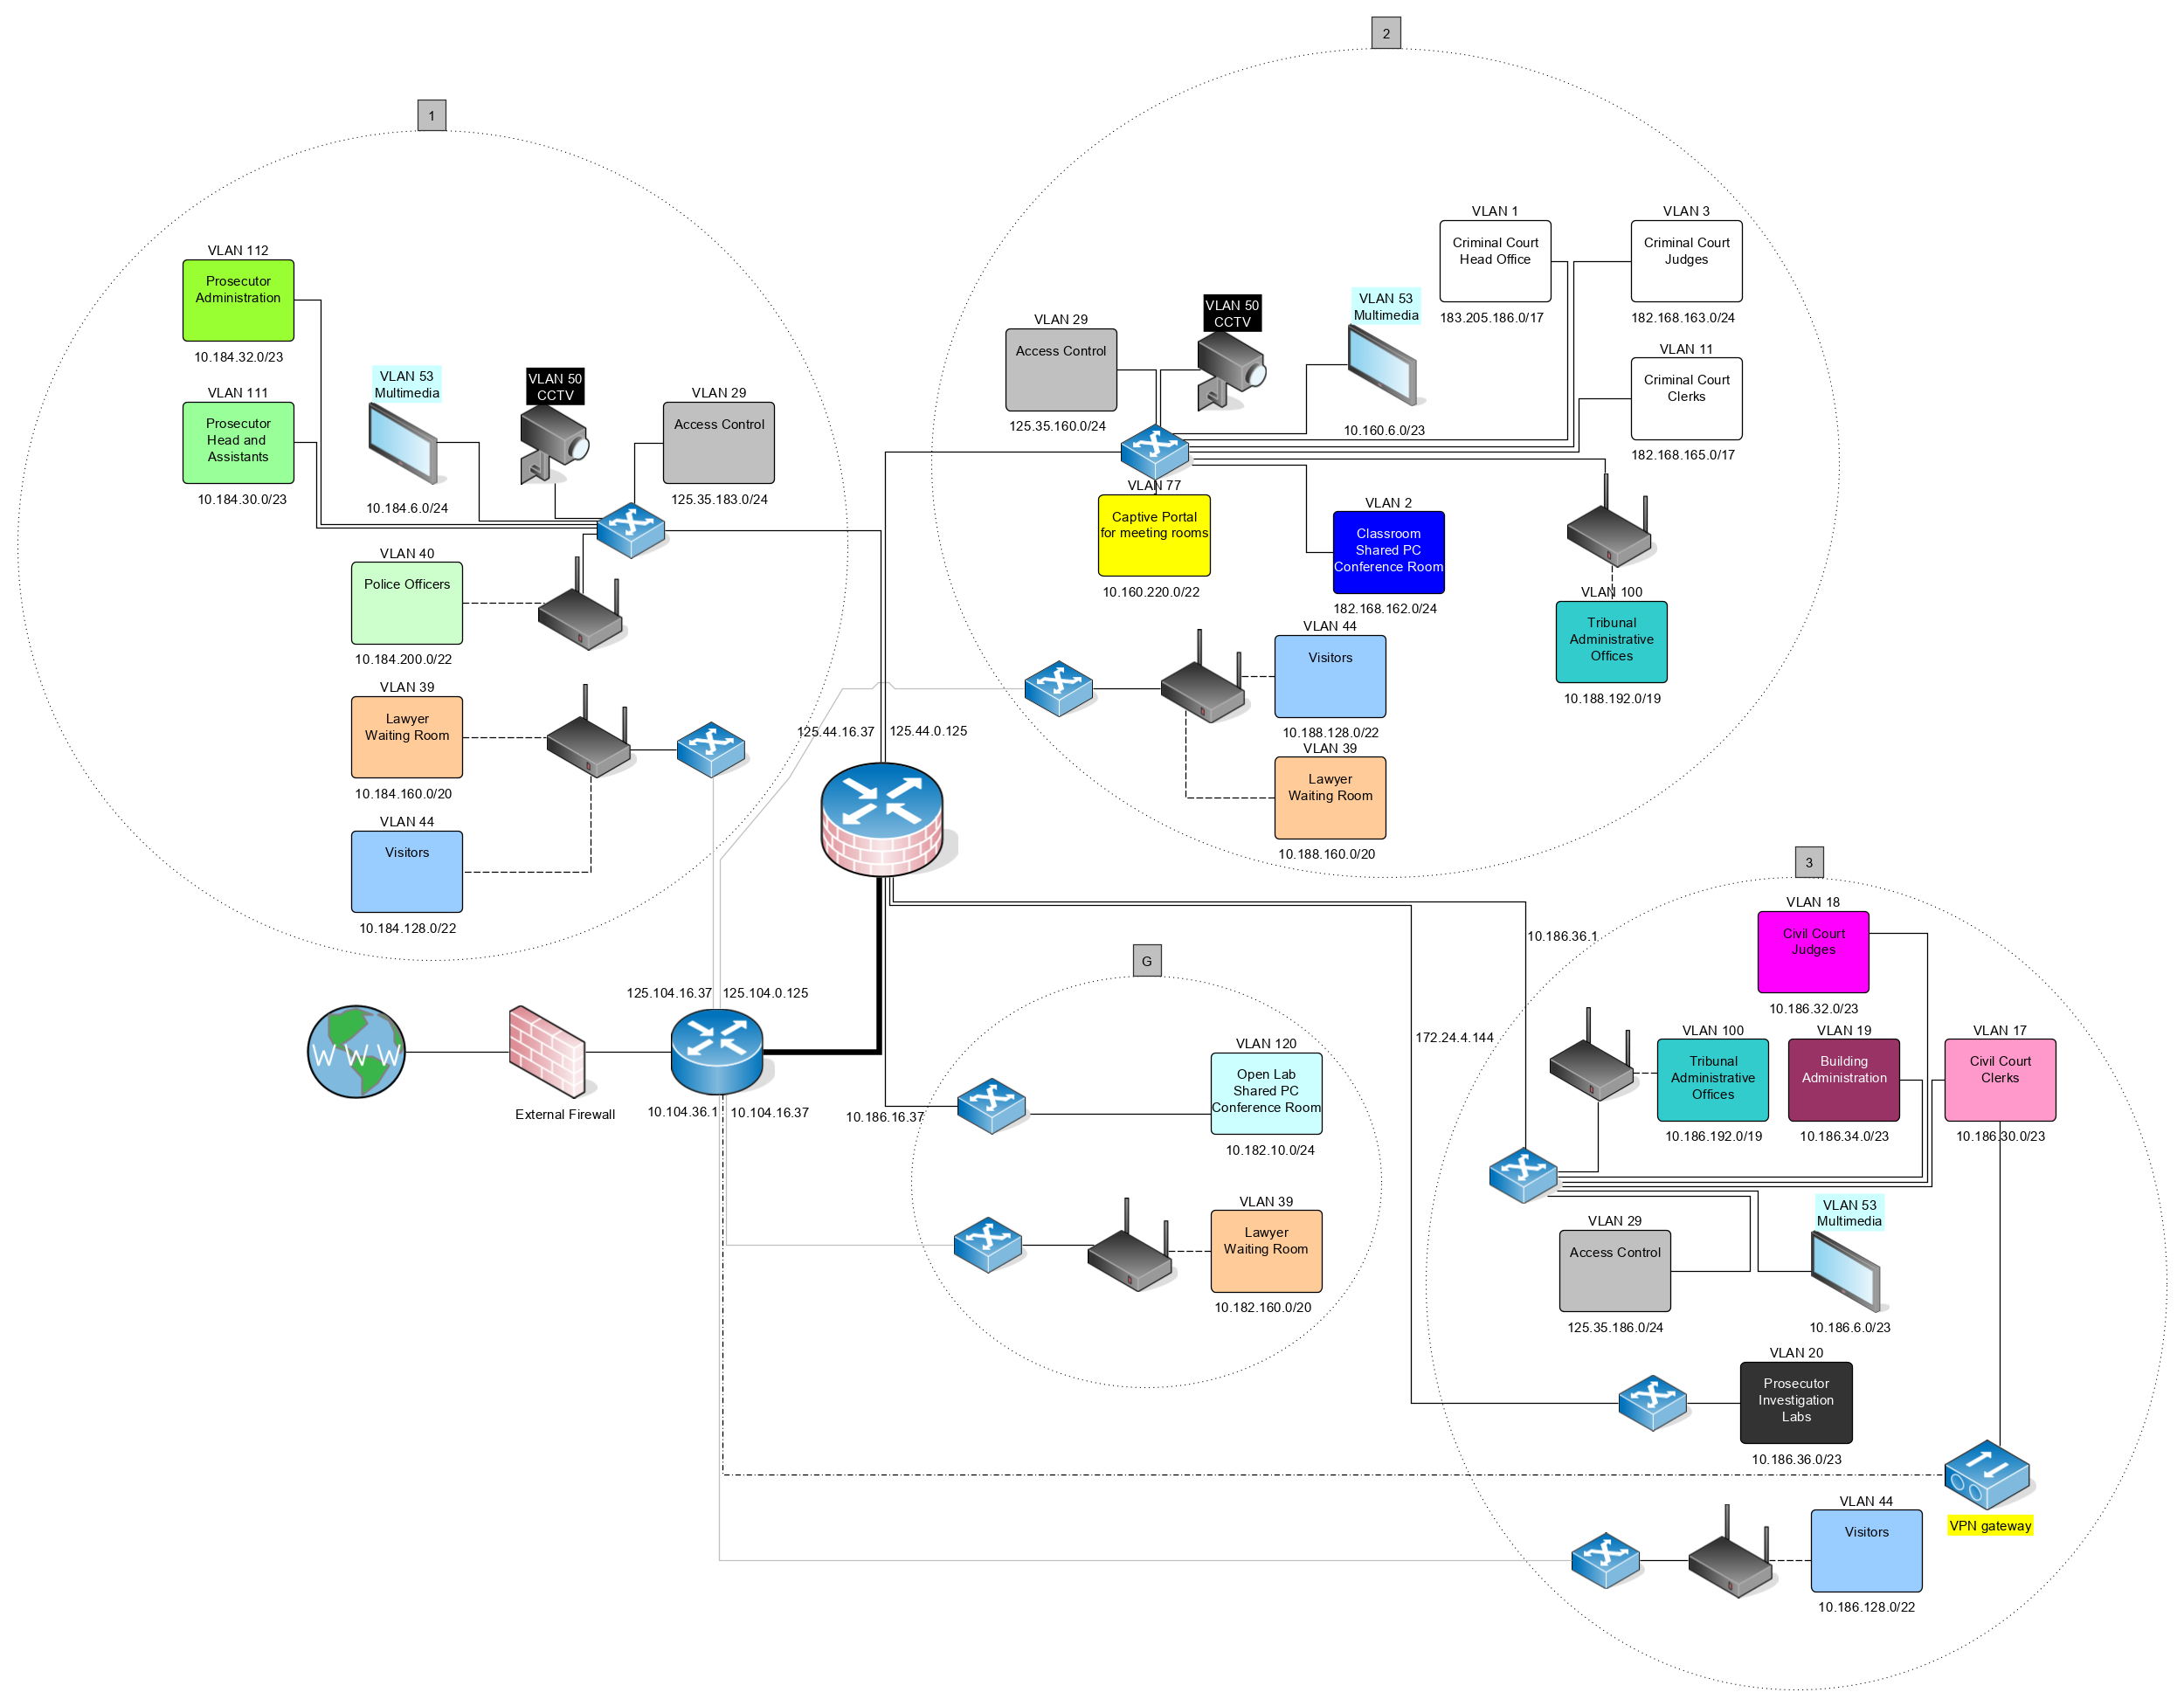
\includegraphics[width=\textwidth]{drawable/rete-updated.png}
	\caption{Architectural Description of the target and the proposed security mitigations to be deployed.}
	\label{fig:updated-network}
\end{figure}

First, we decided to re-number some VLANs as we realized some of them covered completely different sections of the Tribunal. Indeed, VLAN IDs \verb=17= and \verb=18= were shared between the Prosecutors and the Civil Court, and the former were renamed to \verb=111= and \verb=112=. While we do know that inter-VLAN routing should be disabled, we cannot make sure that really there is no route between them, and we want to enforce a "VLAN/IP" policy so that no two subnets share an IP or a VLAN ID. In this case, it was extremely important to segregate them as VLAN \verb=111= was found to be ridden with vulnerabilities in the provided scan.

The same approach was taken for the for the Shared PC Conference Room at ground floor, moved to VLAN \verb=120=, and the Tribunal Administrative Offices, moved to VLAN \verb=100= away from the Police Officers one. We undertook several redesigns of the cable layout, and our best suggestion is to reconfigure the network in order to either use the only firewall as both a gateway firewall and inter-network firewall, or to buy a new apparatus and deploy it such that the communication between any two VLANs is secured. These costs are later discussed in the quantitative analysis. 

We also took steps in order to make sure that subnets related to visitors are not only logically but also physically separated from the rest of the network. Indeed, the scan showed such subnets without a gateway, and we addressed it by creating new fictitious IPs for a gateway located before the central firewall but after the gateway firewall.

\begin{figure}[!h]
	\centering
	%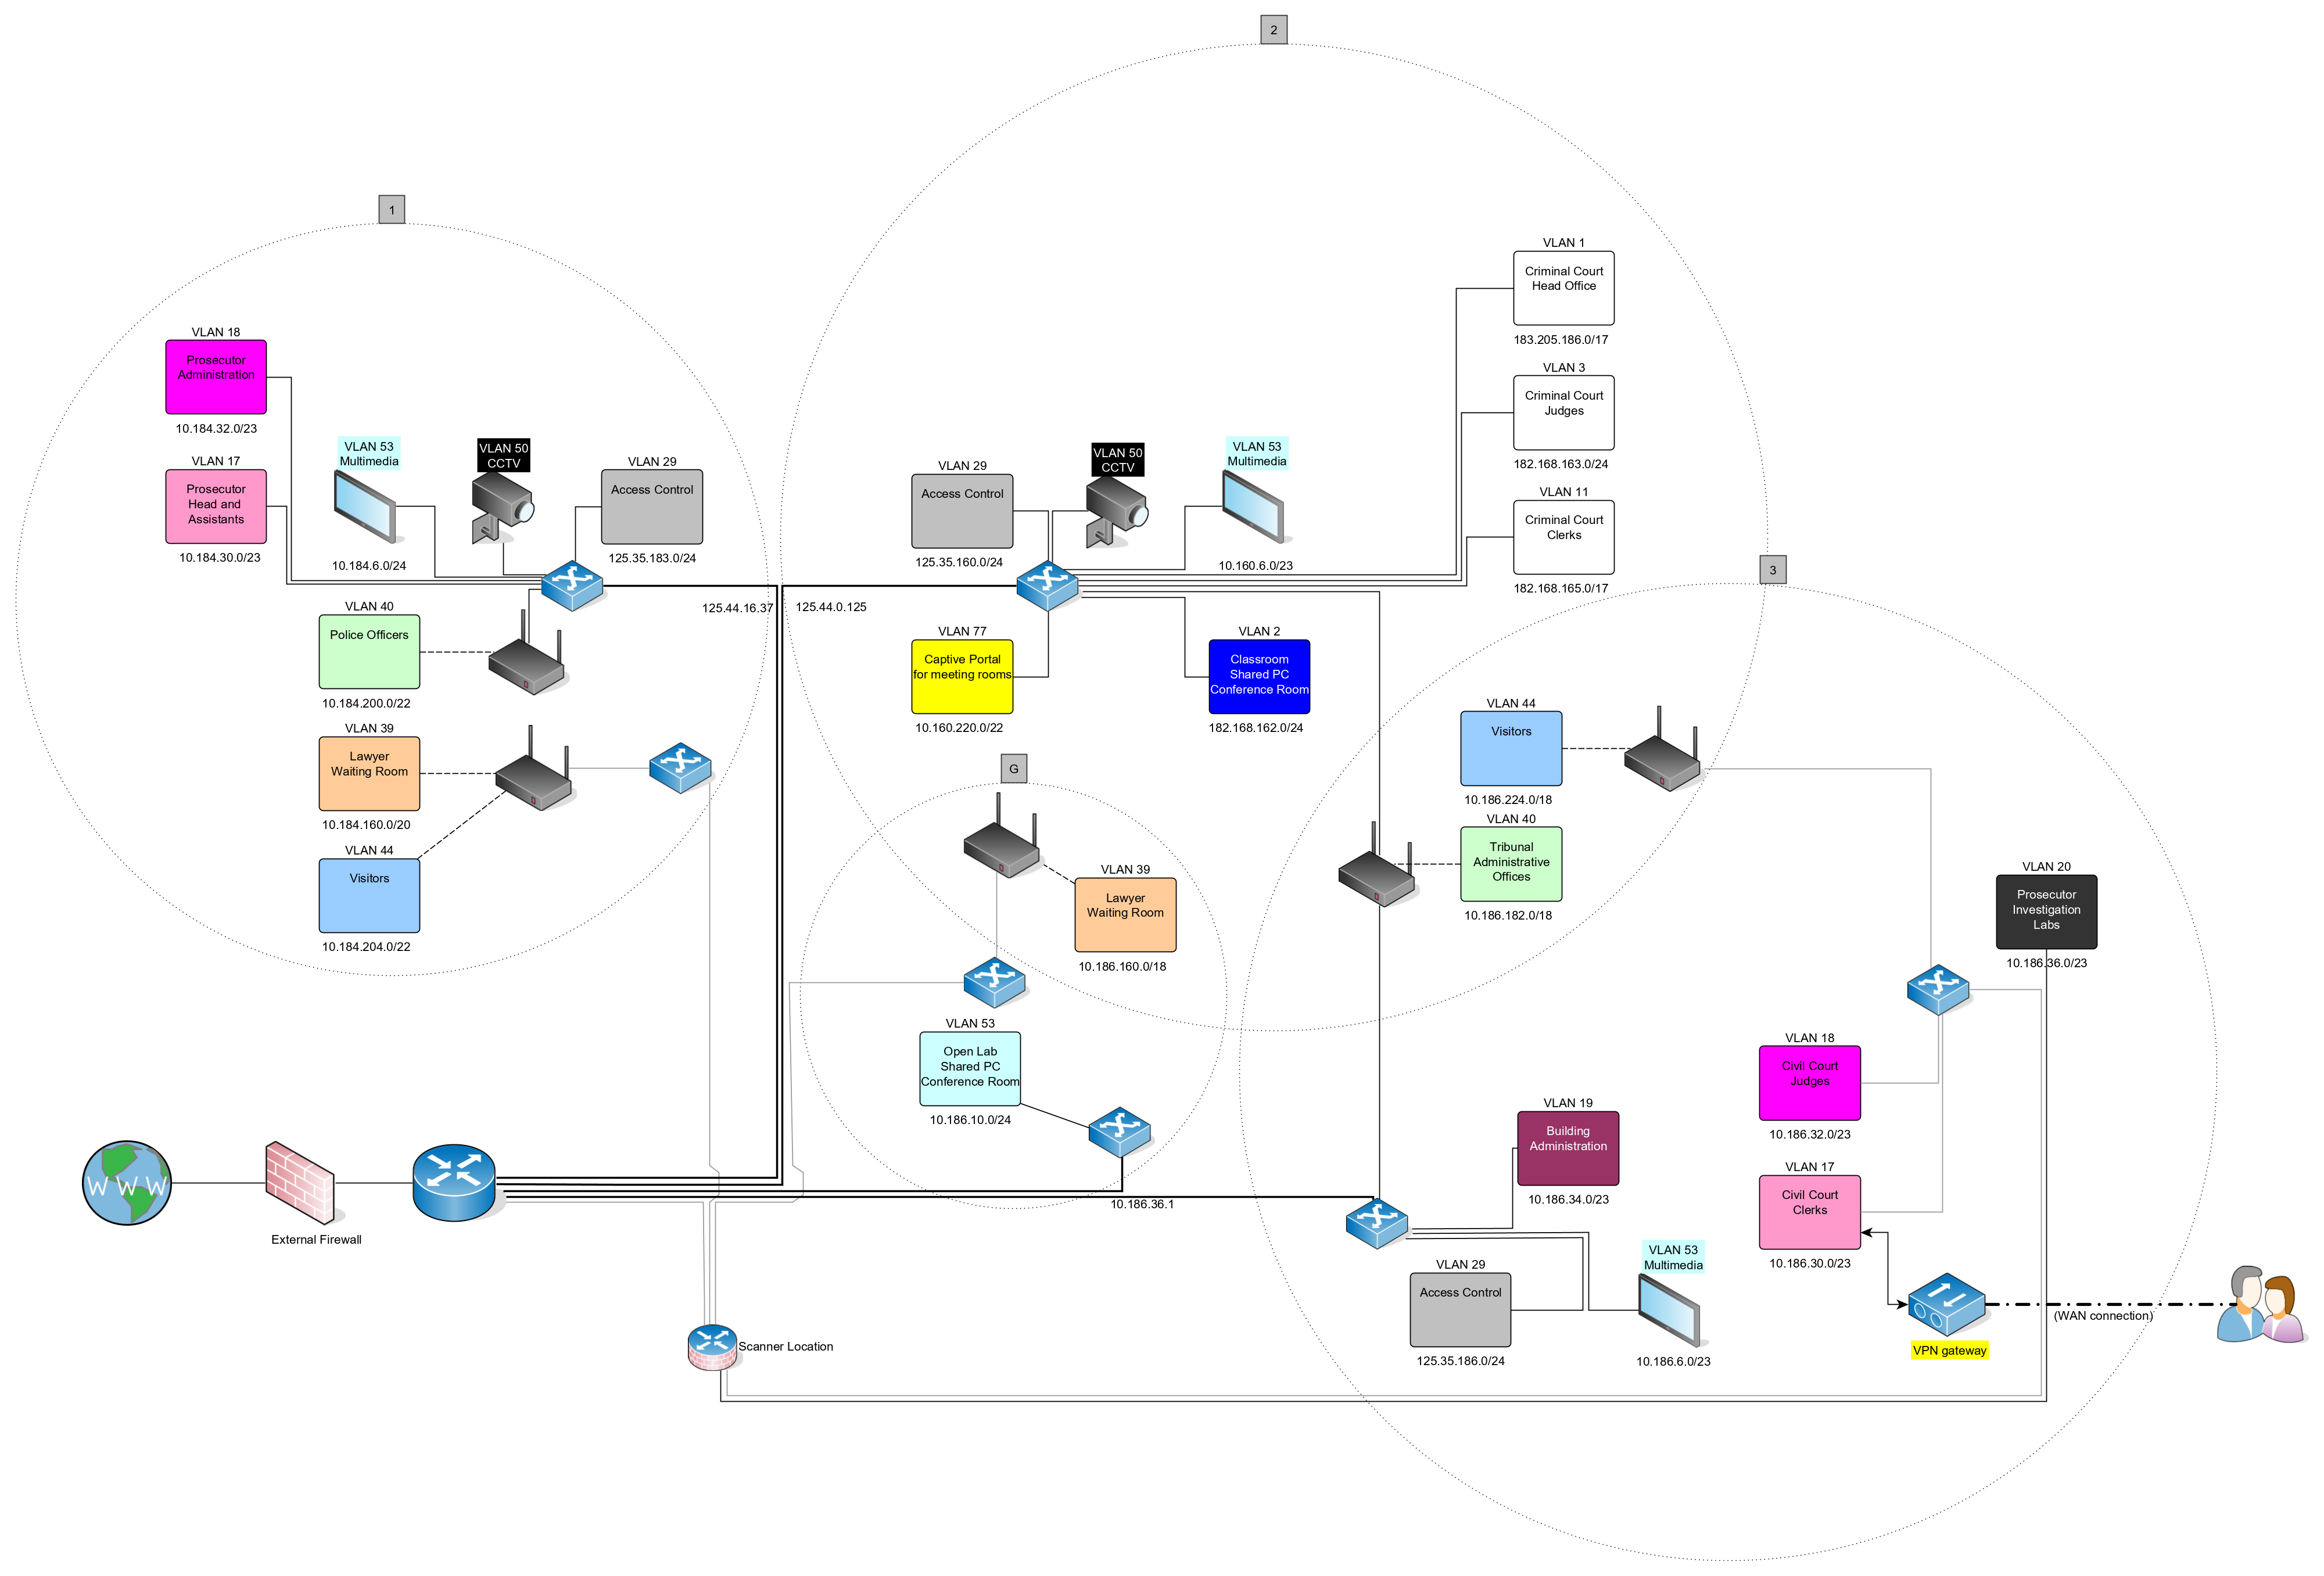
\includegraphics[width=1.4\textwidth]{drawable/rete.png}
	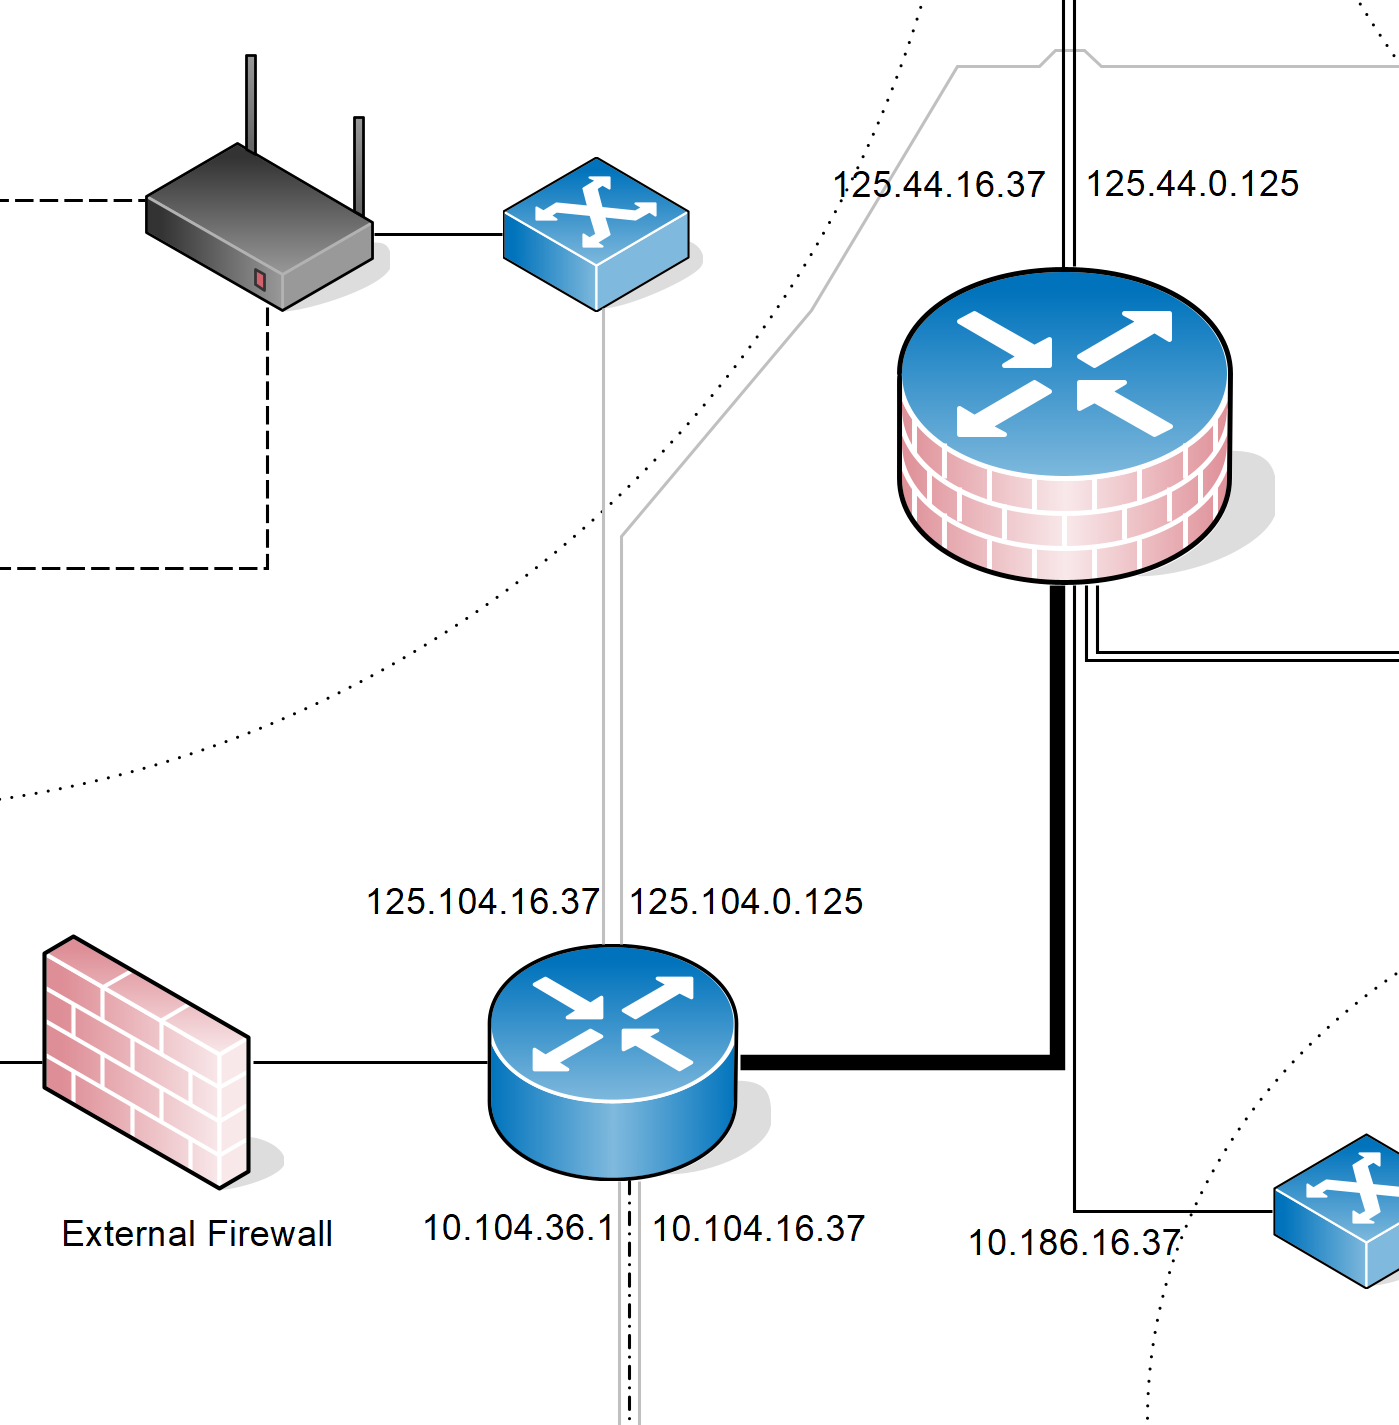
\includegraphics[width=0.5\textwidth]{drawable/detail-network.png}
	\caption{Enlarged snippet of the network diagram. We can see the external firewall, the initial gateway, and the inter-network firewall.}
	\label{fig:detail-network}
\end{figure}

Finally, in the diagram we moved some subnets around and introduced some logic in the IPs. Now, in most subnet IPs, the second group now reflects the floor of the subnet and VLAN itself. This caused the split of two subnets, mainly those related to visitors and hotspot access points. For example, subnet \url{10.186.224.0/19} was split into \url{10.188.128.0/22} and \url{10.186.128.0/22} for the Visitors subnet, with \verb=188= denoting the second floor and \verb=186= denoting the third. In general, this was done in order to avoid some overlapping that were present in the provided list. In the wake of this final suggestion, we also want to promote a full revision of all IPs (as this diagram is only meant to be a guideline) and firewall rules.

\subsection{Main analysis}

After completing our architectural redesign, we focused on the qualitative analysis. Our findings showed that while most supporting assets did have their fair share of High risk, the most at-risk ones were the VPN and log server(s) and the networking devices. This goes to show how fundamental it is and it would become the network architecture if one were to implement the suggested VPN system.

We took prompt action in order to secure and mitigate risk as much as possible. Our main suggested controls include the deployment of guards in the data center, redundancy, automated fail-over detection, and in general methods that allow enforcement of business continuity. We also stressed the need of installing a new inter-network firewall and enforcing employee policy in order to prevent undesirable social engineering attack vectors.

In the end, while the residual risk was almost flattened for some assets such as the VPN server itself, most primary assets did end up with a medium residual risk. However, we believe that it is an acceptable level of risk when taken into account jointly with the proposed quantitative countermeasures.

Indeed, our quantitative analysis focused on the possible monetary impact of several cyber attack scenarios on what we thought we were the most compromised machines in the system. Firstly, we collected the most prominent CVSS vulnerabilities from the provided Nessus scan. Secondly, we identified key systems and assigned IDs to them, enumerating their importance and their CVSS scores. For each of them, we discussed their importance and the probability of it being used as an attack vector for a cyber attack.

We then condensed the obtained data into a table in step 3, contextualizing attacks into five different possible main targets: the external firewall, the judicial software server, the VPN server, the log server, and a Clerk's PC. For each of them, we calculated the impact and the likelihood of an attack, first in a day, then amortized on a year.

Finally, we collected information about our controls implemented in the qualitative report, and researched their cost. After obtaining a reasonable estimate, we used that information to re-do the impact and likelihood calculation with the countermeasures.

What we found out was that due to mainly the GDPR-complying fines, the worst possible scenario would be an attack on the VPN server, with its estimated cost ranging in the tens of millions of euros. Additionally, other sensitive equipment such as the Clerks' PCs and the judicial software server were deemed risky of multi-million incidents. While the countermeasures did sharply decrease such a risk, the residual risk still remains in the same order of magnitude, and is almost impossible to completely mitigate, given the circumstances and the importance of the data managed by the tribunal.

\clearpage